\documentclass[e4_tp1_main.tex]{subfiles}
\begin{document}

\section{Topolog\'ia: Funcionamiento de una topolog\'ia y comprensio\'n de todas las curvas}

\subsection*{a) Diseño de la fuente} 

Se diseñ\'o una fuente con las siguientes caracter\'isticas:

\begin{table}[H]
\centering
\begin{tabular}{|l|l|l|l|l|}
\hline
\multicolumn{1}{|c|}{Grupo}  & $V_{i}$ & $V_{o}$  & $\frac{\Delta V_{o_{max}}}{V_o}$ & $f_{sw}$ \\ \hline
3     						& 5V     & 3.3V  & 5\%   & 60kHz  \\ \hline
\end{tabular}
\label{tabla:datos de la fuente}
\end{table} 



Como se pide una tensi\'on de salida continua menor que a la entrada, se utiliz\'o un convertidor buck. 


\begin{figure}[H]
  \centering
    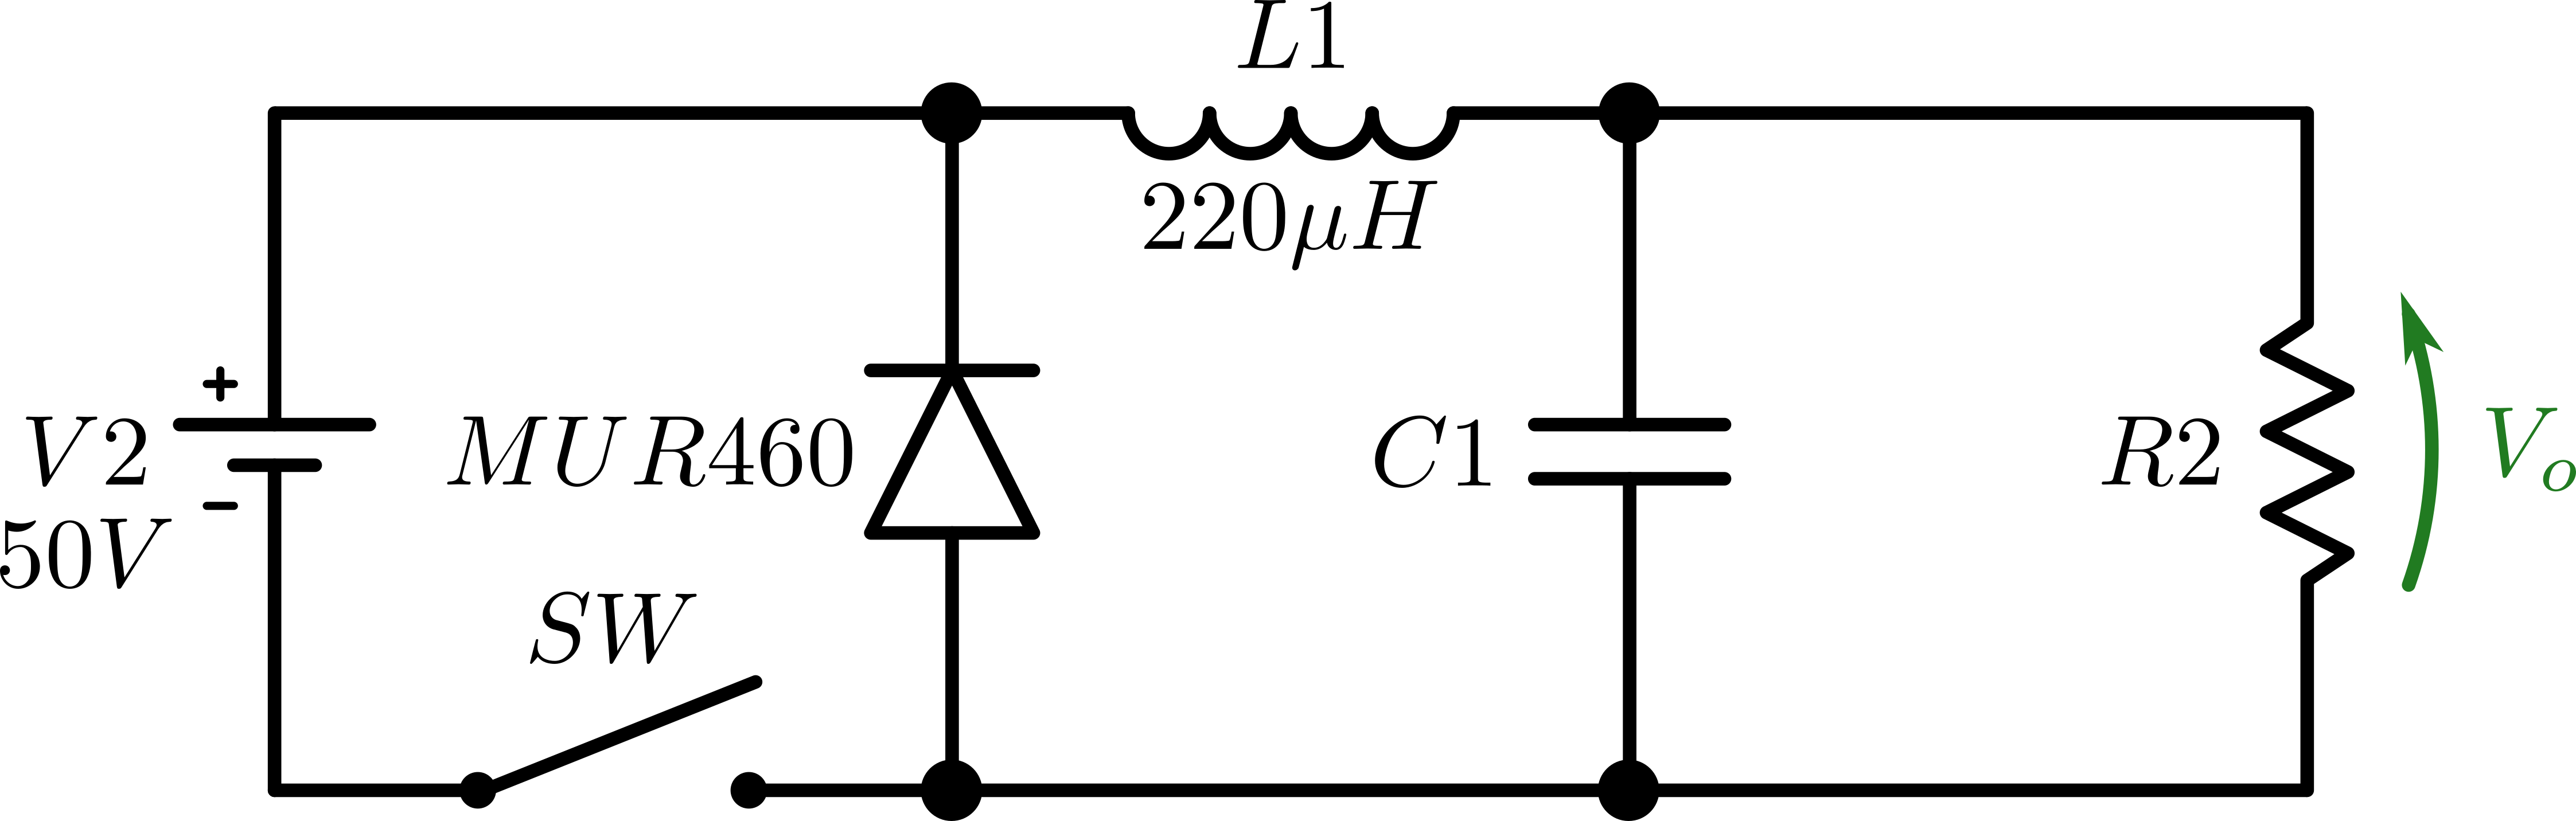
\includegraphics[scale = 0.8]{Imagenes/punto2/Circuito2.png}
  \caption{Buck Converter}
  \label{Circuito}
\end{figure}




Sabemos que el duty cycle en este convertidor esta dado por: 
$$D_{ideal}=\frac{V_o}{V_i}=0.66$$

Con el valor del duty obtenemos el periodo de encendido de la llave $T_{on}=D T_s=D \frac{1}{f_{sw}}$


Para asegurarnos que estemos trabajando en modo continuo, elegimos una $I_{o}$ tal que: $I_{o}>I_{OB}$:

\[
I_{OB}(L=220\mu H) = \frac{V_o \cdot (1-D_{ideal}) \cdot T_s}{2L} = 42.5mA
\]


%Resultando: 

%\begin{table}[H]
%\centering
%\begin{tabular}{|l|l|}
%\hline
%\multicolumn{1}{|c|}{$L [\mu H]$} & {$I_{OB} [mA]$}    \\ \hline
%220                   & 42.5   \\ \hline
%\end{tabular}
%\caption{Calculo de $I_{OB}$ seg\'un el valor de $L$}
%\label{tabla:calculo de Iob}
%\end{table}

Por lo tanto, suponiendo $I_o=100mA$, obtenemos una carga de $R=33\Omega$



El valor del capacitor se obtuvo con la siguiente formula:
$$C=\frac{(1-D_{ideal}) \cdot T_{s}^{2}}{8\cdot L\cdot \frac{\Delta V_{o_{max}}}{V_o}}=1.073\mu F$$

Para realizar las simulaci\'on se tom\'o  $L=220\mu H$ y se obtuvo que: 
$$D_{real}=0.711$$

\newpage

\subsection*{b) Curvas teóricas}

Se realiz\'o el gr\'afico de la señal de disparo (SW), tensión en el inductor (VL),corriente en el inductor (IL) y corriente en el diodo (ID) considerando el diodo real. 

\begin{figure}[H]
  \centering
    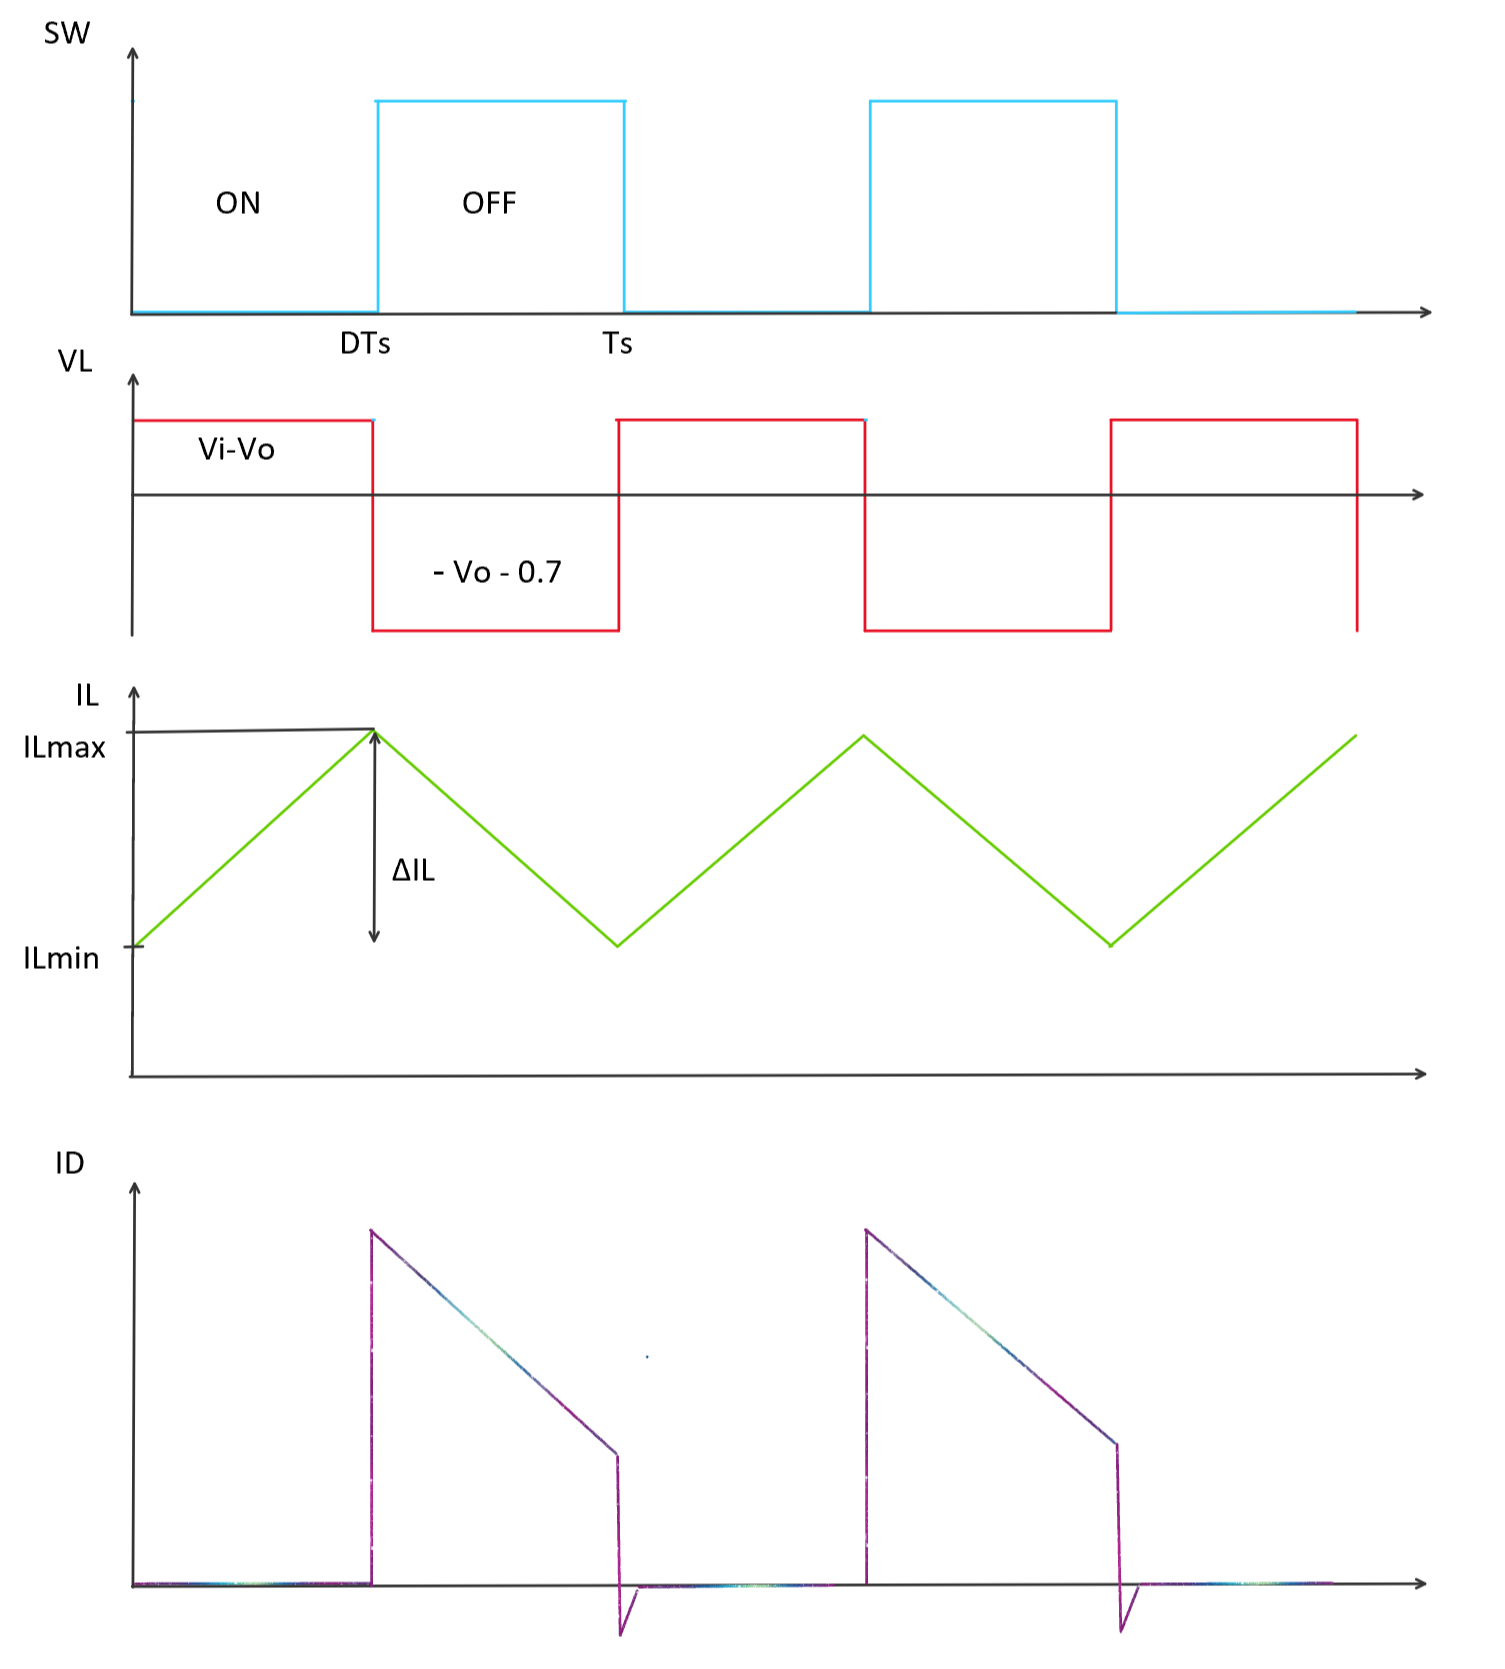
\includegraphics[scale = 0.6]{Imagenes/punto2/Dibujo}
  \caption{Gr\'afico las curvas de la topolog\'ia de convertidor boost}
  \label{fig:dibujo}
\end{figure}


Sabiendo que en este convertidor en particular la corriente media en el inductor es igual a la corriente media a la salida, podemos calcular la corriente m\'axima y m\'inima en el inductor como:

$$I_{L_{max}}= I_o + \frac{\Delta I_L}{2}$$
$$I_{L_{min}}= I_o - \frac{\Delta I_L}{2}$$

Adem\'as, en r\'egimen permanente se cumple: $\Delta I_{L_{ON}}+\Delta I_{L_{OFF}}=0$ y $\Delta I_{L_{ON}}=\frac{(V_i-V_o)\cdot D\cdot T_s}{L}$.

$$I_{L_{max}}= I_o + \frac{(V_i-V_o)\cdot D_{real}\cdot T_s}{L}=145mA$$
$$I_{L_{min}}= I_o - \frac{(V_i-V_o)\cdot D_{real}\cdot T_s}{L}=54mA$$

\newpage

\subsection*{c) Curvas simuladas}

A continuaci\'on se muestra la simulaci\'on en LTspice de las curvas del inciso anterior tomando como tiempo de encendido de la llave a $T_{on}=D_{real}T_s$


\begin{figure}[H]
  \centering
    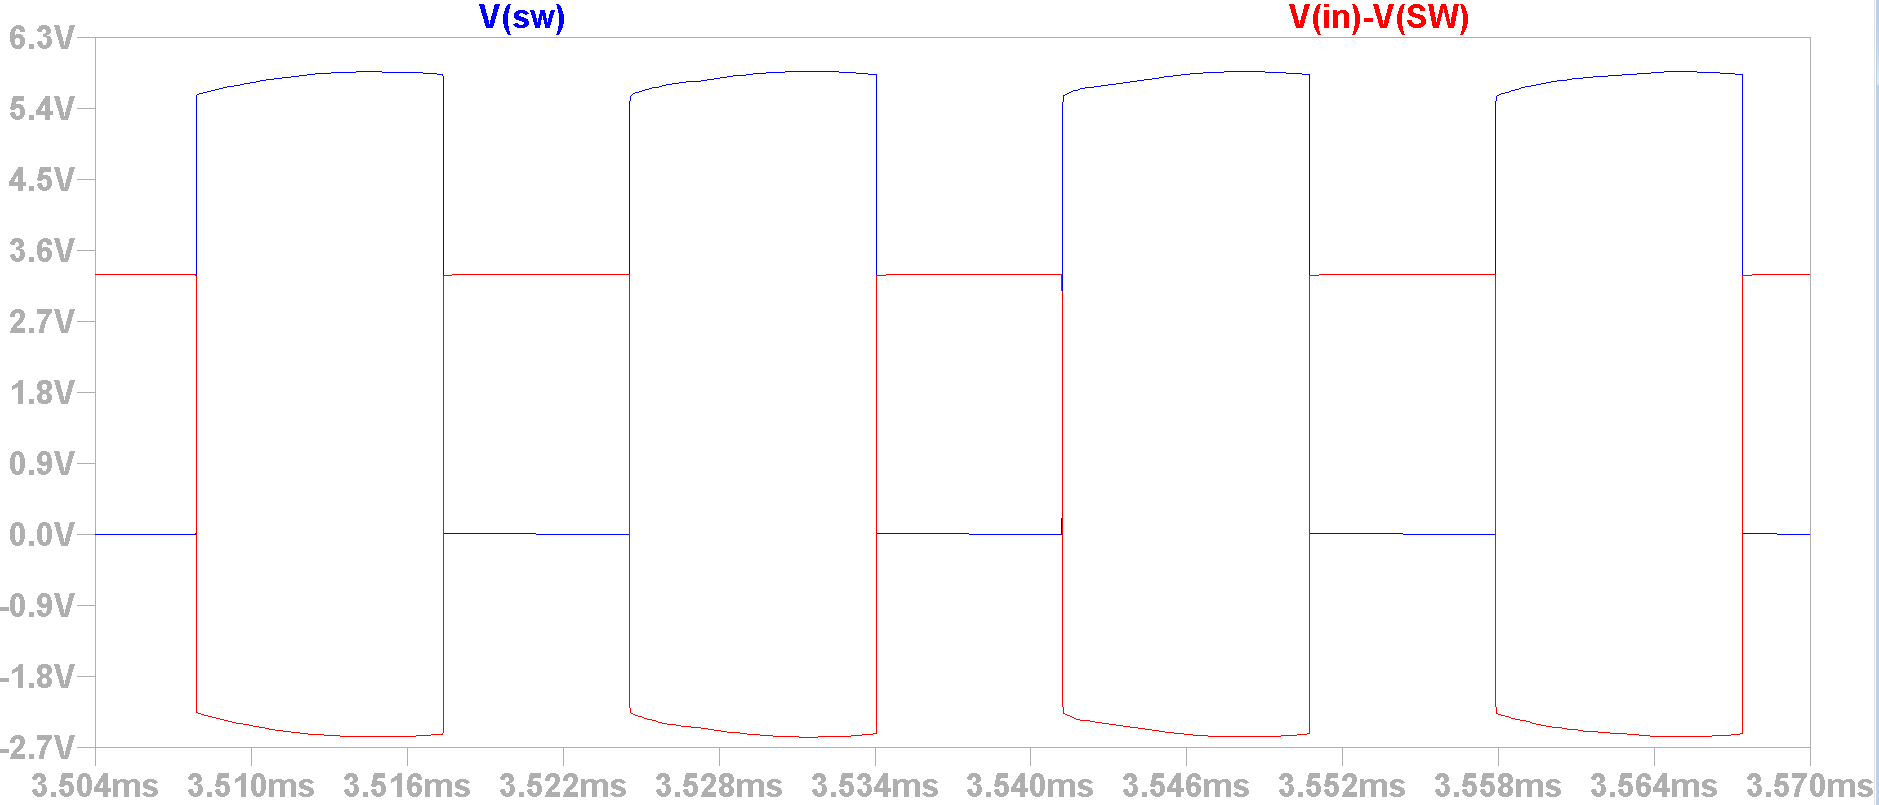
\includegraphics[scale = 0.6]{Imagenes/punto2/SW&VL}
  \caption{Simulaci\'on SW(roja) y VL(azul)}
  \label{fig:SW&VL}
\end{figure}

\begin{figure}[H]
  \centering
    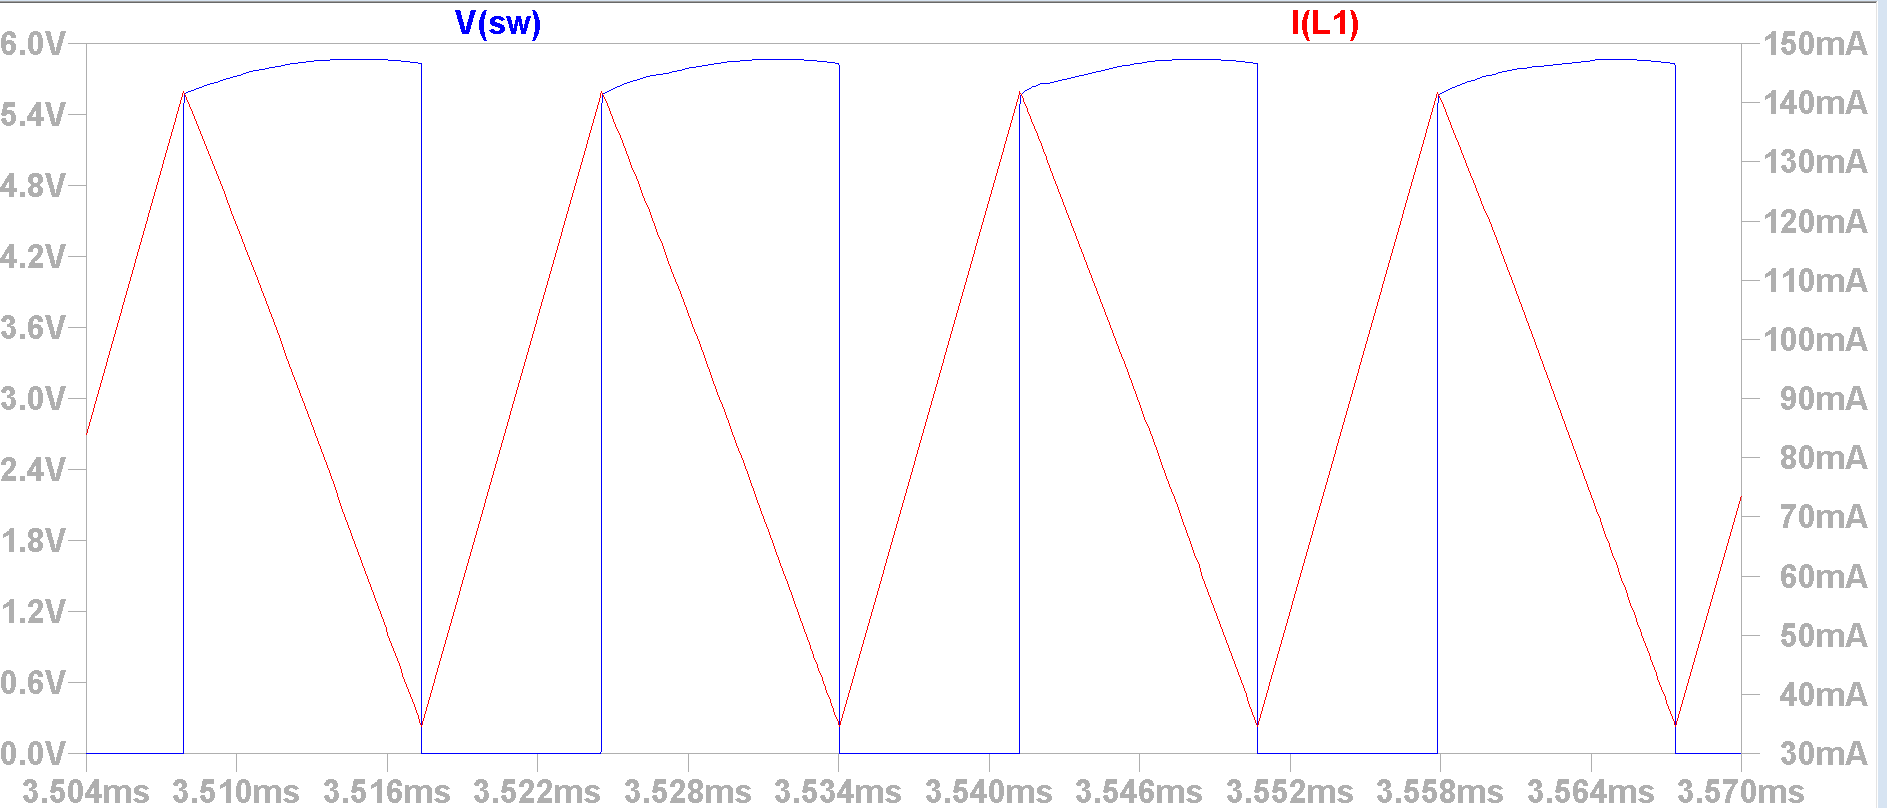
\includegraphics[scale = 0.6]{Imagenes/punto2/SW&IL}
  \caption{Simulaci\'on SW(azul) y IL(verde)}
  \label{fig:SW&IL}
\end{figure}


\begin{figure}[H]
  \centering
    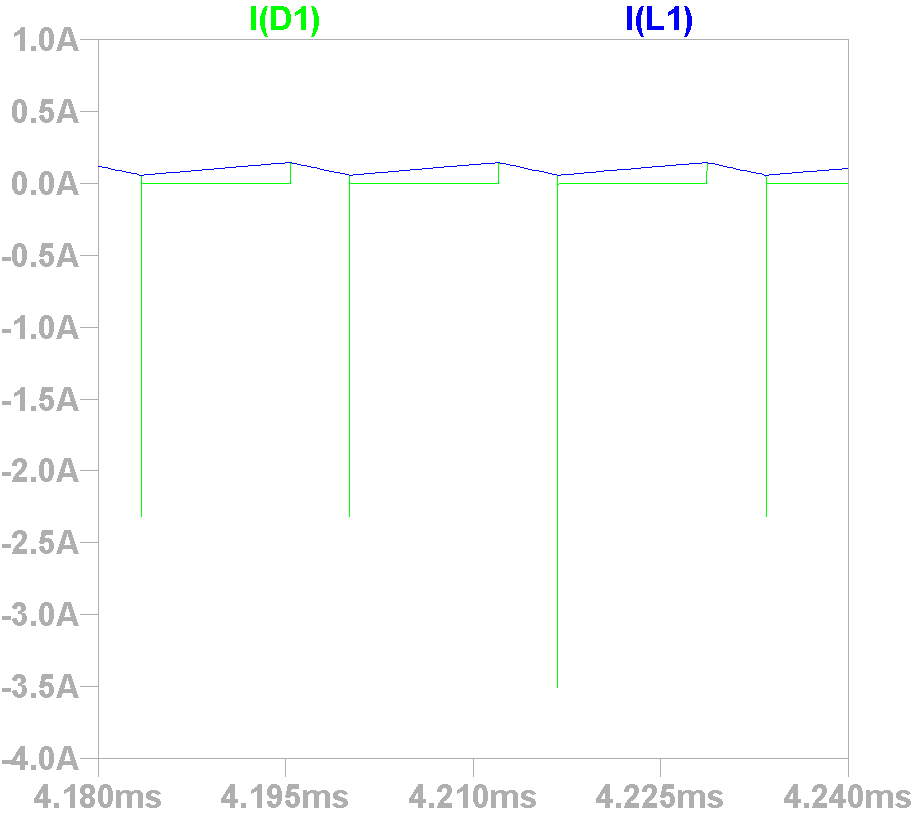
\includegraphics[scale=1]{Imagenes/punto2/PicodeIrr}
  \caption{Simulaci\'on IL(azul) y ID(verde)}
  \label{fig:IL&ID}
\end{figure}



\begin{figure}[H]
  \centering
    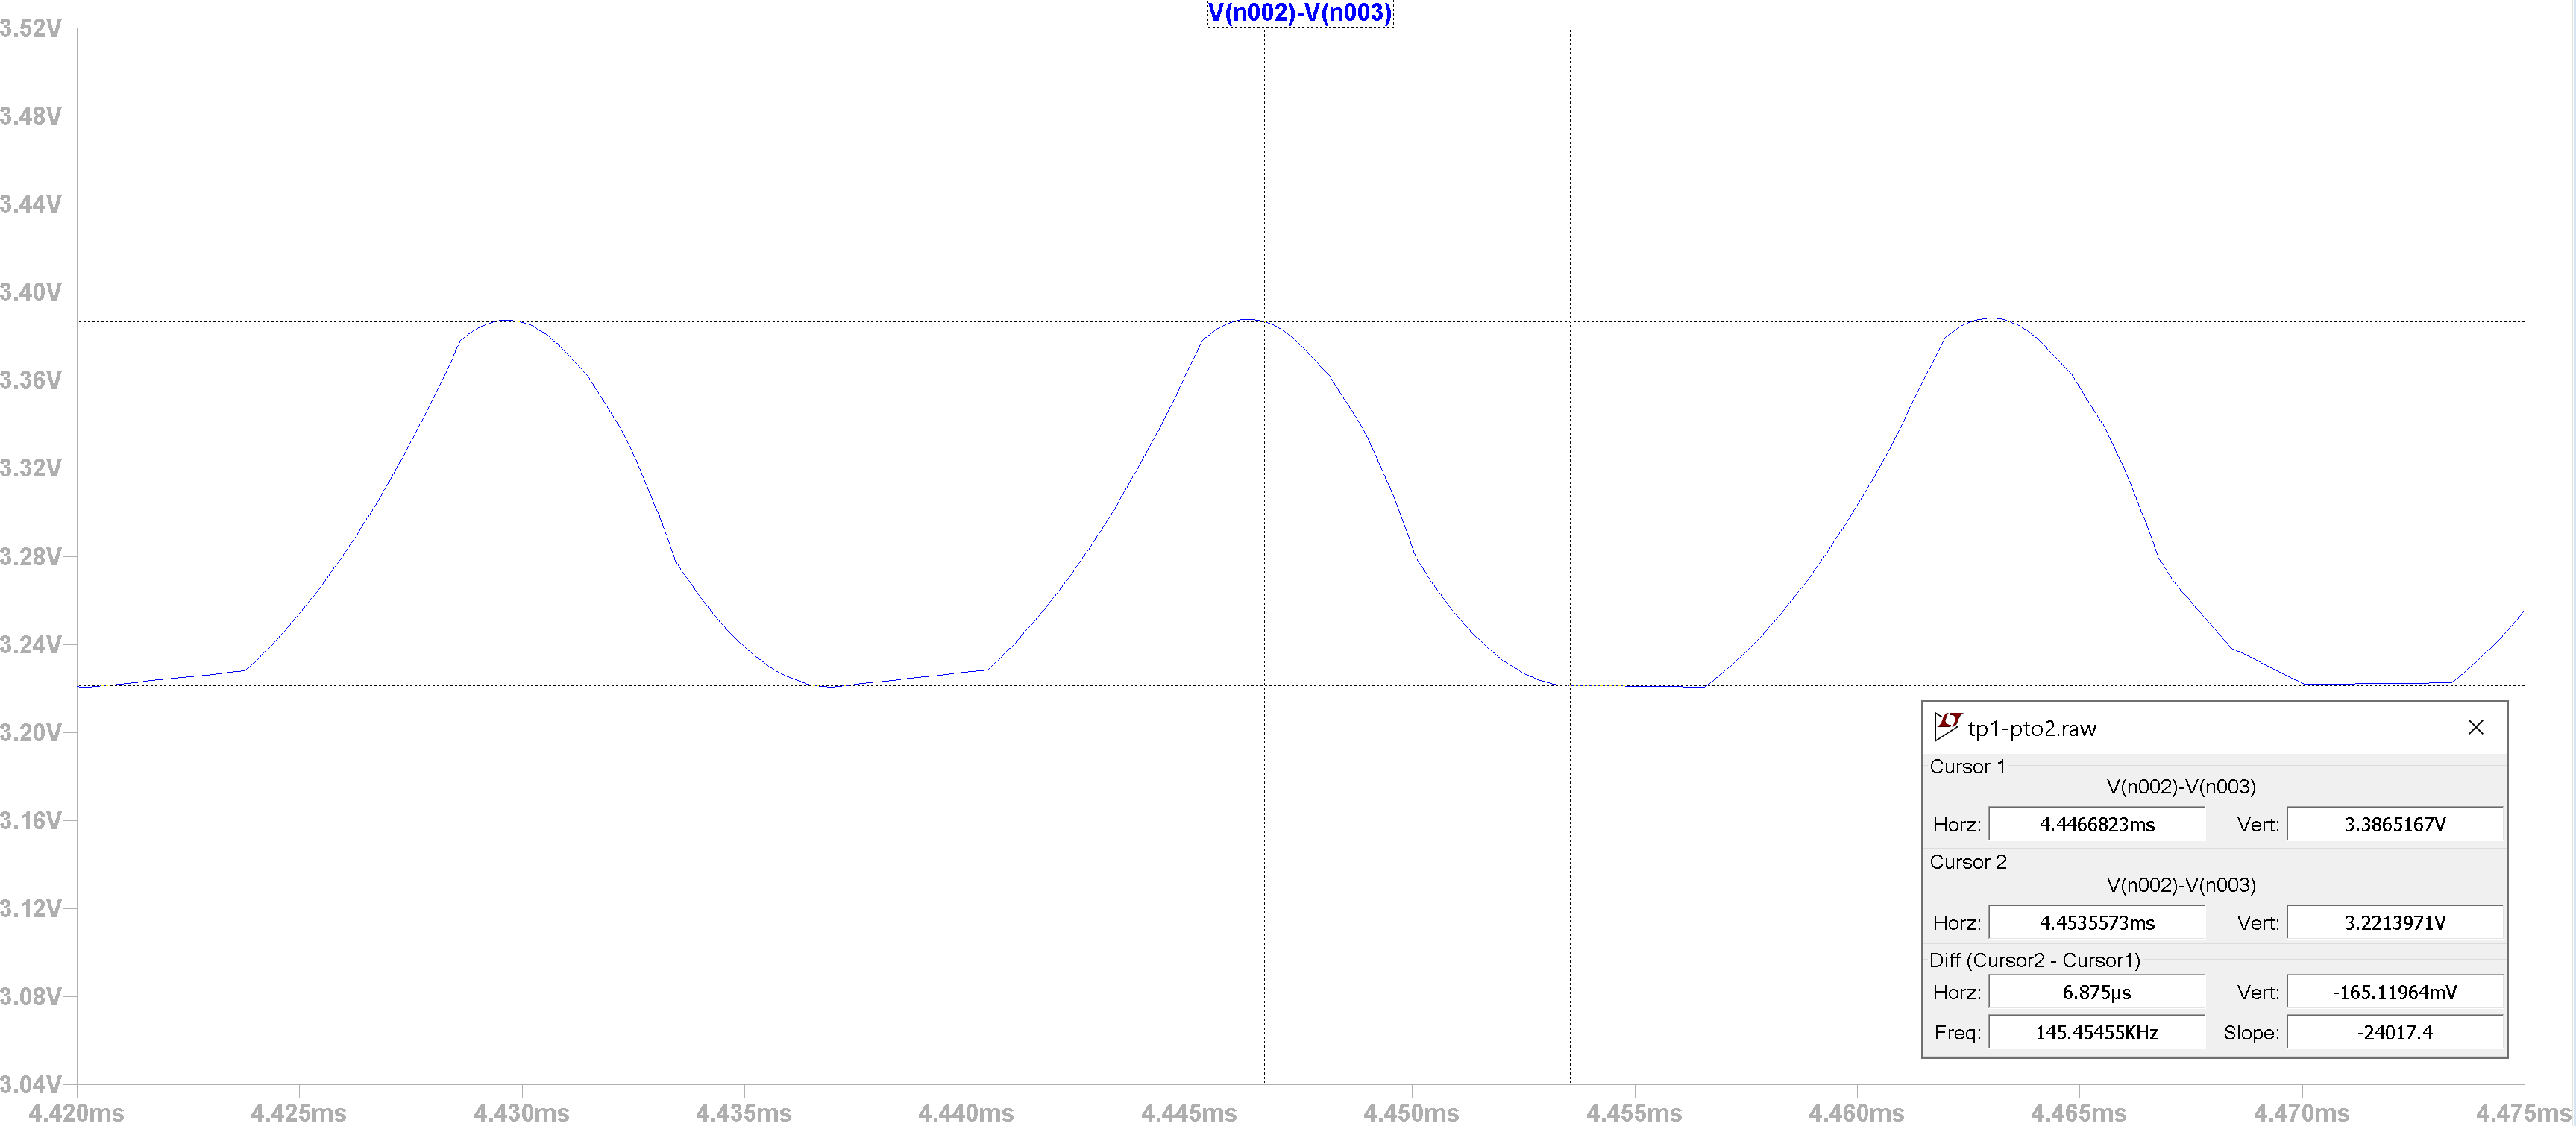
\includegraphics[scale = 0.2]{Imagenes/punto2/Vo-D=0,711.PNG}
  \caption{Simulaci\'on $V_o$ (azul)}
  \label{fig:IL&ID}
\end{figure}

\subsection*{d) Comparaciones y observaciones}

En los c\'alculos que se realizaron en el inciso a) se consider\'o al diodo como ideal. Si tenemos en cuenta la ca\'ida del diodo cuando conduce, la tensi\'on en el inductor mientras $SW=OFF$ es $V_{L}=V_o(Teorica)-V_{forw}$, o sea cercana a $2,6V$. Por ello se debió aumentar el duty del circuito para alcanzar la $V_o$ deseada (como se menciona más abajo). Mismo ocurre con la tensión sobre el SW: cuando está abierto, resulta la tensión de la fuente más la caída del diodo, llegando a los $5,7V$.\par 
Adem\'as, debemos considerar el pico de corriente de reverse recovery $(I_{rr})$ cuando el diodo deja de conducir. En el gráfico teórico se la señalo como un pico inverso menor, pero en la simulación se verificó que resulta ser bastante mayor, pudiendo llegar a mostrae hasta un valor de 3A. Dado que el SW es ideal, durante este tiempo es como si se produjera un cortocircuito en la fuente, por lo que es razonable que la simulación muestre un valor grande. En la práctica, el pico que se produzca (que en este caso pasa a través del SW) tendrá que soportarlo el transistor MOS, como se experimentará en la sección 3. 



Como la tensi\'on $V_L$ se ve afectada por el comportamiento no ideal del diodo, tambi\'en se ver\'a afectada el $D_{ideal}$ calculado.
Cuando realizamos la simulaci\'on con un $T_{on}=D_{ideal}T_s$, la tensi\'on de salida se encontraba por debajo de los 3.3V. Por dicho motivo, aumentamos $D$ hasta lograr la tensi\'on de salida deseada. 

Considerando el ripple que nos agreg\'o la ESR del capacitor, obtuvimos que el $D$ que cumple con los requerimientos de nuestra fuente es $D_{real}=0.711$, mayor al estimado en forma teórica, $D_{ideal} = 0.66$.

El ripple que se obtiene a la salida, considerando una $ESR_C=1\Omega$ es un $\Delta V_o = 165mV$, que equivale al $5\%$ buscado.






\newpage
\end{document}